
\subsection{mCVaR-based optimization strategies}\label{S:mCVaR}

This section presents portfolio optimization strategies based on the mixture \CVaR\ dispersion measure, \ie,
\begin{equation}
    \mCVaR = \sum_{l=1}^{L} \cK_l \times \CVaR_{\alpha_l},
    \label{cvar0}
\end{equation}
where $\{\cK_l\}_{l=1,\cdots,L}$ is a set of positive coefficients normalized to unit (the mixture coefficients),
$\{\alpha_l\}_{l=1,\cdots,L}$ is a set of distinct confidence levels and
\begin{equation}
    \CVaR_\alpha(X) = \min_u\left[u + \frac{1}{1-\alpha}\mE\left[(-\bX-u)^+\right] \right],
    \label{cvarS}
\end{equation}
where $\bX = X - \mE[X]$.

On the side note, \mCVaR\ can be viewed as a particular case of
a Spectral measure \cite{Acerbi}.

\BackToContents


\subsubsection{mCVaR dispersion measure}

We start by listing the main result from Rockafaller and Uryasev \cite{Uryasev}.
Given a set of observed rates of returns, $\{r_i\}_{i=1,\cdots,N}$,
the \CVaR\ from Eq.~(\ref{cvarS}) can be rewritten as
\begin{equation}
    \CVaR_\alpha = \min_u\left[ u +  \frac{1}{(1-\alpha)N} \sum_{i=1}^N \left(-u -\br_i \right)^+ \right],
    \label{cvar1:1}
\end{equation}
where $\br_i = r_i - \frac{1}{N}\sum_{j=1}^N r_j$ are the detrended historical observations and
$\alpha$ is the confidence level.\footnote{A typical value could be 0.975, then \CVaR\ is the
average return of the 2.5 percentile.}


It is straightforward to show that, Eq~(\ref{cvar1:1}) can be transformed into the
following LP problem.

\bigskip
\noindent Minimize over $\{u, \{s_i\}_{i=1,\cdots,N}\}$
\begin{subequations}\label{cvar1}
\begin{align}
    &g = u + \frac{1}{(1-\alpha) N} \sum_{i=1}^N s_i, \label{cvar1a} \\
    \st & s_i + u \geq - \br_i, \label{cvar1b} \\
        & s_i \geq 0, \label{cvar1c} \\
        & u \geq 0. \label{cvar1d}
\end{align}
\end{subequations}

\noindent Then, we have
\begin{subequations}\label{cvar2}
\begin{align}
    \CVaR_\alpha &= g^*, \label{cvar2a} \\
    \VaR_\alpha &= u^*, \label{cvar2b}
\end{align}
\end{subequations}

\noindent where $^*$ denotes the solution of LP problem.


The LP problem from Eqs.~(\ref{cvar1}) has an analytical solution. It can be described as follows.

\bigskip
\noindent Let $\{x_i\}_{i=1,\cdot,N}$
be $\{\br_i\}_{i=1,\cdot,N}$ sorted in ascending order. Then, we have
\begin{subequations}\label{cvar3}
\begin{align}
    \CVaR &= \frac{k^* - a}{a} x_{k^*} - \frac{1}{a} \sum_{i=1}^{k^*} x_i, \label{cvar3a} \\
    \VaR &= x_{k^*}, \label{cvar3b}
\end{align}
\end{subequations}
where
\begin{subequations}\label{cvar4}
\begin{align}
    a &= N(1-\alpha), \label{cvar4a} \\
    k^* &= \lceil a \rceil. \label{cvar4b}
\end{align}
\end{subequations}

\noindent Here $\lceil\cdot\rceil$ denotes the ceiling operator.
A sketched proof of this result is in Appendix~\ref{AppendixA}.

\noindent Further, \mCVaR\ is given by the sum from Eq.~(\ref{cvar0}).

Form a numerical point of view, the implementation of the analytic solution is preferred over the LP algorithm.
This approach has been implemented in the \azapy\ package.
However, the transformation of Eq.~(\ref{cvar1:1})
into the LP problem from Eqs.~(\ref{cvar1}) is at the core of all LP formulations for \mCVaR-based optimal portfolio strategies.
There are no analytical solutions for these LP problems.
Therefore, the numerical algorithms for optimizations must involve LP solvers.

\BackToContents

\subsubsection{mCVaR optimal portfolio}

Formally, this optimization is described by Eqs.~(\ref{gg1}) from Sec.~\ref{strategies} point~\ref{OptRisk},
where $\rho$ is given by the \mCVaR\ from Eq.\ (\ref{cvar0}).
It is straightforward to show that, this optimization is given by the following LP problem.

\bigskip
\noindent Minimize over $\{\{w_k\}_{k=1,\cdots,M}, \{ u_l, \{s_{li}\}_{i=1,\cdots,N}\}_{l=1,\cdots,L}\}$
\begin{subequations}\label{cvar5}
\begin{align}
    &g = \sum_{l=1}^{L}\cK_l \left( u_l + \frac{1}{(1-\alpha_l)N} \sum_{i=1}^N s_{li} \right), \label{cvar5a} \\
    \st &s_{li} + u_l + \sum_{k=1}^M w_k \br_{ki} \geq 0, \label{cvar5b} \\
        &\sum_{k=1}^M w_k \mu_k \geq \mu, \label{cvar5c} \\
        &\sum_{k=1}^M w_k = 1, \label{cvar5d} \\
        & s_{li} \geq 0, \label{cvar5e} \\
        & u_l \geq 0, \label{cvar5f} \\
        & w_k \geq 0, \label{cvar5g}
\end{align}
\end{subequations}

\noindent where $\mu$ from Eq.~(\ref{cvar5c}) is the portfolio targeted expected rate of return, while $\{\mu_k\}_{k = 1,\cdots,M}$
are the portfolio components expected rate of return. Here, $\br_{ki}$ is the $i$-th detrended\footnote{After
the subtraction of their average, \ie\ $\br_{ki} = r_{ki} - \frac{1}{N}\sum_{j=1}^N r_{kj}$.} observation of the
$k$-th portfolio component rate of return.
Then, we have
\begin{subequations}\label{cvar6}
\begin{align}
    \mCVaR &= g^*, \label{cvar6a} \\
    \RR &= \sum_{k=1}^M w_k^* \mu_k, \label{cvar6b} \\
    \CVaR_{\alpha_l} &= u_l^* + \frac{1}{(1-\alpha_l)N} \sum_{i=1}^N s_{li}^*, \label{cvar6c} \\
    \VaR_{\alpha_l} &= u_l^*, \label{cvar6d}
\end{align}
\end{subequations}

\noindent where the $^*$ denotes the solution of LP problem.
In addition to the optimal portfolio weights $\{w_k^*\}_{k=1,\cdots,M}$
and the portfolio expected rate of return $\RR$,
the LP solution provides information about the portfolio \mCVaR\ and its  \CVaR\
and associated \VaR\ components.


\bigskip
\noindent Here is an example, using the \azapy\ package, of how to compute the \mCVaR\ optimal portfolio.
The \mCVaR\ time horizon was set to one quarter and the calibration is performed using the prior 3.25 years of
close-adjusted historical prices (default settings).
For more details see the package documentation at \azapydoc.

\lstinputlisting[language=Python]{../PyScripts/CVaR_RiskOptim.py}

\BackToContents

\subsubsection{Minimum mCVaR portfolio}

Following the results from Sec.~\ref{strategies} point~\ref{MinRisk},
the algorithm to compute the optimal portfolio with minimum \mCVaR\ is given by the LP problem from Eqs.~(\ref{cvar5}) where
$\mu$ from r.h.s. of Eq.~(\ref{cvar5c}) is set to a value equal to the smallest expected rate of
return among the portfolio components, \ie\ $\mu = \min_k\{\mu_k\}$.

\bigskip
\noindent Here is an example, using the \azapy\ package, of how to compute the minimum \mCVaR\ portfolio.
The \mCVaR\ time horizon was set to one quarter and the calibration is performed using the prior 3.25 years of
close-adjusted historical prices (default settings).
For more details see the package documentation at \azapydoc.

\lstinputlisting[language=Python]{../PyScripts/CVaR_MinRisk.py}

\BackToContents

\subsubsection{mCVaR optimal portfolio for targeted risk value}

This optimization is described by Eqs.~(\ref{gg2}) from Sec.~\ref{strategies} point~\ref{TargetRisk},
where $\rho$ is given by the \mCVaR\ from Eq.~(\ref{cvar0}).
It is the following LP problem.

\bigskip
\noindent Maximize over $\{ \{w_k\}_{k=1,\cdots,M}, \{ u_l, \{ s_{li}\}_{i=1,\cdots,N} \}_{l=1,\cdots, L}\}$
\begin{subequations}\label{cvar7}
\begin{align}
    &g = \sum_{k=1}^M w_k \mu_k, \label{cvar7a} \\
    \st & \sum_{l=1}^L \cK_l \left( u_l + \frac{1}{(1-\alpha_l) N} \sum_{i=1}^N s_{li} \right) = \mCVaR_0, \label{cvar7c} \\
        &s_{li} + u_l + \sum_{k=1}^M w_k \br_{ki} \geq 0, \label{cvar7b} \\
        & \sum_{k=1}^M w_k = 1, \label{cvar7d} \\
        & s_{li} \geq 0, \label{cvar7e} \\
        & u_l \geq 0, \label{cvar7f} \\
        & w_k \geq 0, \label{cvar7g}
\end{align}
\end{subequations}

\noindent where $\mCVaR_0$ in Eq.~(\ref{cvar7c}) is the portfolio targeted \mCVaR\ dispersion value.
Then, we have
\begin{subequations}\label{cvar8}
\begin{align}
    \RR &= g^*, \label{cvar8a} \\
    \CVaR_{\alpha_l} &= u_l^* + \frac{1}{(1-\alpha_l) N}\sum_{i=1}^N s_{li}^*, \label{cavr8b} \\
    \VaR_{\alpha_l} &= u_l^*, \label{cvar8c}
\end{align}
\end{subequations}

\noindent where $^*$ denotes the solution of LP problem.
In addition to the optimal portfolio weights $\{w_k^*\}_{k=1,\cdots,M}$ and the portfolio expected rate of return $\RR$,
the LP solution provides information about the \CVaR\ and associated \VaR\ components of $\mCVaR_0$,
although, this information is likely to be known at the outset.

\bigskip
\noindent Here is an example, using the \azapy\ package, of how to compute the optimal portfolio
with the same \mCVaR\ as the equal weighted portfolio.
The \mCVaR\ time horizon was set to one quarter and the calibration is performed using the prior 3.25 years of
close-adjusted historical prices (default settings).
For more details see the package documentation at \azapydoc.

\lstinputlisting[language=Python]{../PyScripts/CVaR_InvNrisk.py}

\BackToContents

\subsubsection{mCVaR optimal portfolio for fixed risk-aversion factor}
This optimization is described by Eqs.~(\ref{gg3}) from Sec.~\ref{strategies} point~\ref{RiskAverse},
where $\rho$ is given by \mCVaR\ from Eq.~(\ref{cvar0}).
It is the following LP problem.

\bigskip
\noindent Maximize over $\{\{w_k\}_{k=1,\cdots,M}, \{ u_l, \{s_{li}\}_{i=1,\cdots,N}\}_{l=1,\cdots,L}\}$
\begin{subequations}\label{cvar9}
\begin{align}
    &g = \sum_{k=1}^M w_k \mu_k - \lambda \sum_{l=1}^{L}\cK_l \left( u_l + \frac{1}{(1-\alpha_l)N} \sum_{i=1}^N s_{li} \right), \label{cvar9a} \\
    \st &s_{li} + u_l + \sum_{k=1}^M w_k \br_{ki} \geq 0, \label{cvar9b} \\
        &\sum_{k=1}^M w_k = 1, \label{cvar9c} \\
        & s_{li} \geq 0, \label{cvar9d} \\
        & u_l \geq 0, \label{cvar9e} \\
        & w_k \geq 0, \label{cvar9f}
\end{align}
\end{subequations}

\noindent where $\lambda$ from Eqs.~(\ref{cvar9a}) is the risk-aversion factor.
Then, we have
\begin{subequations}\label{cvar10}
\begin{align}
    \RR &= \sum_{k=1}^M w_k^* \mu_k, \label{cvar10a} \\
    \mCVaR &= \frac{\RR - g^*}{\lambda}, \label{cvar10b} \\
    \CVaR_{\alpha_l} &= u_l^* + \frac{1}{(1-\alpha_l)N} \sum_{i=1}^N s_{li}^*, \label{cvar10c} \\
    \VaR_{\alpha_l} &= u_l^*, \label{cvar10d}
\end{align}
\end{subequations}

\noindent where $^*$ denotes the solution of LP problem.
In addition to the optimal portfolio weights $\{w_k^*\}_{k=1,\cdots,M}$ and the portfolio expected rate of return $\RR$,
the LP solution provides information about the portfolio \mCVaR\ and its \CVaR\  and associated \VaR\ components.

\bigskip
\noindent Here is an example, using the \azapy\ package, of how to compute the optimal portfolio
for a given value of the risk-aversion factor $\lambda$.
The \mCVaR\ time horizon was set to one quarter and the calibration is performed using the prior 3.25 years of
close-adjusted historical prices (default settings).
For more details see the package documentation at \azapydoc.

\lstinputlisting[language=Python]{../PyScripts/CVaR_Averse.py}

\BackToContents

\subsubsection{mCVaR-Sharpe optimal portfolio - maximization solution}
This optimization targets the maximization of \mCVaR-Sharpe
ratio.\footnote{\mCVaR-Sharpe ratio is defined by Eq.~(\ref{ggg}) where $\rho=\mCVaR$.}
It is based on the Eqs.~(\ref{gg4}) from Sec.~\ref{strategies} point~\ref{MaxSharpe},
where $\rho$ is given by the \mCVaR\ from Eq.~(\ref{cvar0}).
The optimization can be formulated as an LP problem if Eq.~(\ref{gg4b}) can be linearized.
In our case the linearization is straightforward. Introducing the
variable transformations $\bw_k = t w_k$, $\bs_{li} = t s_{li}$ and $\bu_l = t u_l$, the LP
problem can be written as follows.

\bigskip
\noindent Maximize over $\{\{\bw_k\}_{k=1,\cdots,M}, \{ \bu_l, \{\bs_{li}\}_{i=1,\cdots,N}\}_{l=1,\cdots,L}, t\}$
\begin{subequations}\label{cvar11}
\begin{align}
    &g = \sum_{i=1}^M \bw_k \mu_k - \mu_0 t, \label{cvar11a} \\
    \st &\sum_{l=1}^L \cK_l \left( \bu_l + \frac{1}{(1 - \alpha_l) N} \sum_{i=1}^N \bs_{li} \right) = 1, \label{cvar11d} \\
        &\bs_{li} + \bu_l + \sum_{k=1}^M \bw_k \br_{ki} \geq 0, \label{cvar11b} \\
        &\sum_{k=1}^M \bw_k - t = 0, \label{cvar11c} \\
        &t \geq 0, \label{cvar11h} \\
        &\bs_{li} \geq 0, \label{cvar11e} \\
        &\bu_l \geq 0, \label{cvar11f} \\
        &\bw_k \geq 0, \label{cvar11g}
\end{align}
\end{subequations}

\noindent where $\mu_0$ from Eq.~(\ref{cvar11a}) is the risk-free rate accessible to the investor.
Then, we have
\begin{subequations}\label{cvar12}
\begin{align}
    w_k &= \frac{\bw_k^*}{t^*} , \label{cvar12a} \\
    \RR &= \frac{g^*}{t^*}  + \mu_0, \label{cvar12b} \\
    \Sharpe & = g^*, \label{cvar12c} \\
    \mCVaR &= \frac{1}{t^*}, \label{cvar12d} \\
    \CVaR_{\alpha_l} &= \frac{1}{t^*} \left( \bu_l^* + \frac{1}{(1 - \alpha_l) N} \sum_{i=1}^N \bs_{li}^* \right), \label{cvar12e} \\
    \VaR_{\alpha_l} &= \frac{\bu_l^*}{t^*} , \label{cvar12f}
\end{align}
\end{subequations}

\noindent where $^*$ denotes the solution of LP problem.
In addition to the optimal portfolio weights $\{w_k\}_{k=1,\cdots,M}$, expected rate of return $\RR$ and \mCVaR-Sharpe ratio $\Sharpe$,
the LP solution provides information about the portfolio \mCVaR\ and its \CVaR\  and associated \VaR\ components.

\bigskip
\noindent Here is an example, using the \azapy\ package, of how to compute the \mCVaR-Sharpe optimal portfolio using the maximization
of \mCVaR-Sharpe ratio.
The \mCVaR\ time horizon was set to one quarter and the calibration is performed using the prior 3.25 years of
close-adjusted historical prices (default settings).
For more details see the package documentation at \azapydoc.

\lstinputlisting[language=Python]{../PyScripts/CVaR_Sharpe.py}

\BackToContents

\subsubsection{mCVaR-Sharpe optimal portfolio - minimization solution}
This optimization targets the minimization of the inverse of \mCVaR-Sharpe ratio.
It is  described by Eqs.~(\ref{gg8}) from Sec.~\ref{strategies} point~\ref{MinSharpe}, where
$\rho$ is given by \mCVaR\ from Eq.~(\ref{cvar0}).
The optimization can be formulated as an LP problem if Eq.~(\ref{gg8a}) can be linearized. This can be achieved by
introducing the following variable transformations
$\bw_k = t w_k$, $\bs_{li} = t s_{li}$ and $\bu_l = t u_l$.
Then, the LP problem can be written as follows.

\bigskip
\noindent Minimize over $\{\{\bw_k\}_{k=1,\cdots,M}, \{ \bu_l, \{\bs_{li}\}_{i=1,\cdots,N}\}_{l=1,\cdots,L}, t\}$
\begin{subequations}\label{cvar13}
\begin{align}
    &g = \sum_{l=1}^L \cK_l \left( \bu_l + \frac{1}{(1 - \alpha_l) N} \sum_{i=1}^N \bs_{li} \right), \label{cvar13a} \\
    \st &\sum_{k=1}^M \bw_k \mu_k - t\mu_0 = 1, \label{cvar13c} \\
        &\bs_{li} + \bu_l + \sum_{k=1}^M \bw_k \br_{ki} \geq 0, \label{cvar13b} \\
        &\sum_{k=1}^M \bw_k - t = 0, \label{cvar13d} \\
        &t \geq 0, \label{cvar13h} \\
        &\bs_{li} \geq 0, \label{cvar13e} \\
        &\bu_l \geq 0, \label{cvar13f} \\
        &\bw_k \geq 0, \label{cvar13g}
\end{align}
\end{subequations}

\noindent where $\mu_0$ from Eq.~(\ref{cvar13c}) is the risk-free rate accessible to the investor.
Then, we have
\begin{subequations}\label{cvar14}
\begin{align}
    w_k &= \frac{\bw_k^*}{t^*} , \label{cvar14a} \\
    \RR &= \frac{1}{t^*} + \mu_0, \label{cvar14b} \\
    \Sharpe &= \frac{1}{g^*}, \label{cvar14c} \\
    \mCVaR &= \frac{g^*}{t^*} , \label{cvar14d} \\
    \CVaR_{\alpha_l} &= \frac{1}{t^*} \left( \bu_l^* + \frac{1}{(1 - \alpha_l) N} \sum_{i=1}^N \bs_{li}^* \right), \label{cvar14e} \\
    \VaR_{\alpha_l} &= \frac{\bu_l^*}{t^*} , \label{cvar14f}
\end{align}
\end{subequations}

\noindent where $^*$ denotes the solution of LP problem.
In addition to the optimal portfolio weights $\{w_k\}_{k=1,\cdots,M}$, expected rate of return $\RR$ and \mCVaR-Sharpe ratio $\Sharpe$,
the LP solution provides information about the portfolio \mCVaR\ and its \CVaR\  and associated \VaR\ components.

\bigskip
\noindent Here is an example, using the \azapy\ package, of how to compute the \mCVaR-Sharpe optimal portfolio using the minimization
of the inverse of \mCVaR-Sharpe ratio.
The \mCVaR\ time horizon was set to one quarter and the calibration is performed using the prior 3.25 years of
close-adjusted historical prices (default settings).
For more details see the package documentation at \azapydoc.

\lstinputlisting[language=Python]{../PyScripts/CVaR_InvSharpe.py}

\BackToContents

\subsubsection{mCVaR frontiers}

Here is an example of how to compute the \mCVaR\ frontiers using the \azapy\
package. The \mCVaR\ time horizon was set to one quarter and the calibration is performed using the prior 3.25 years of
close-adjusted historical prices (default settings).
For more details see the package documentation at \azapydoc.

The script produces the plots in Figs.~\ref{CVaR_fig1a} and \ref{CVaR_fig1b}
for historical data collected up to 2021-07-27.

\lstinputlisting[language=Python]{../PyScripts/CVaR_frontiers.py}

\begin{figure}[H]
\centering
\begin{subfigure}{.5\textwidth}
  \centering
  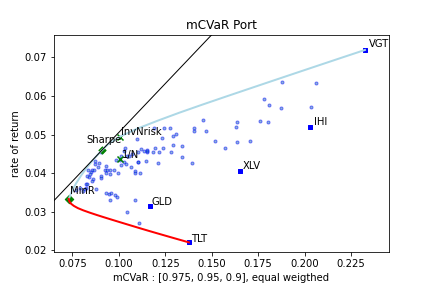
\includegraphics[width=.95\linewidth]{../figs/mCVaRFrontier1.png}
  \caption{Rate of return vs. \mCVaR}
  \label{CVaR_fig1a}
\end{subfigure}%
\begin{subfigure}{.5\textwidth}
  \centering
  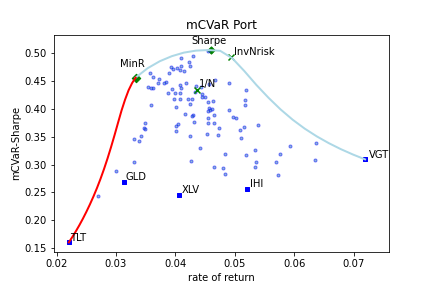
\includegraphics[width=.95\linewidth]{../figs/mCVaRFrontier2.png}
  \caption{\mCVaR-Sharpe vs. rate of return}
  \label{CVaR_fig1b}
\end{subfigure}
\caption{\mCVaR\ : [$\alpha=(0.975, 0.95, 0.9)$, equal weighted] frontiers.}
\label{CVaR_fig1}
\end{figure}

\BackToContents

\subsubsection{Backtesting mCVaR-Sharpe optimal portfolio}

Here is an example, using \azapy\ package, of computing a portfolio backtesting.
For this example, we have chosen a portfolio quarterly rebalanced according
to the maximization of \mCVaR-Sharpe ratio. At each rebalancing date,
the portfolio weights
are calibrated based on 3.25 years of prior historical market data (default settings).

Other rebalancing strategies can be considered
by changing the value of {\it rtype} parameter in the call of {\it set\_model} function below.
For more details see the package documentation at \azapydoc.

\lstinputlisting[language=Python]{../PyScripts/CVaR_Port.py}

\begin{figure}[H]
    \centering
    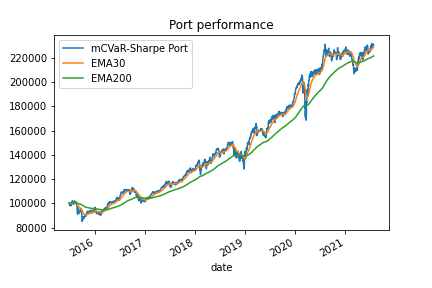
\includegraphics[width=.95\linewidth]{../figs/Port_mCVaR_Sharpe.png}
    \caption{Backtesting of quarterly rebalanced \mCVaR-Sharpe optimal portfolio,
    \mCVaR\ : [$\alpha=(0.975, 0.95, 0.9)$, equal weighted].}
    \label{CVaR_Port_fig}
\end{figure}

\BackToContents 